\documentclass[]{article}
\usepackage{graphicx}
\graphicspath{ {./images/} }

%opening
\title{Appendix}
\author{Zixuan Huang}

\begin{document}

\maketitle

According to the results in Aiyagari(1994), the differences between the saving rates with an without insurance are quite small for moderate and empirically plausible values of $\sigma$, $\rho$, and $\mu$. However for high values of $\sigma$, $\rho$, and $\mu$, the presence of idiosyncratic risk can raise the saving rate quite significantly. \\

The table below is extracted from Aiyagari(1994) and clearly shows this point. 

\centering
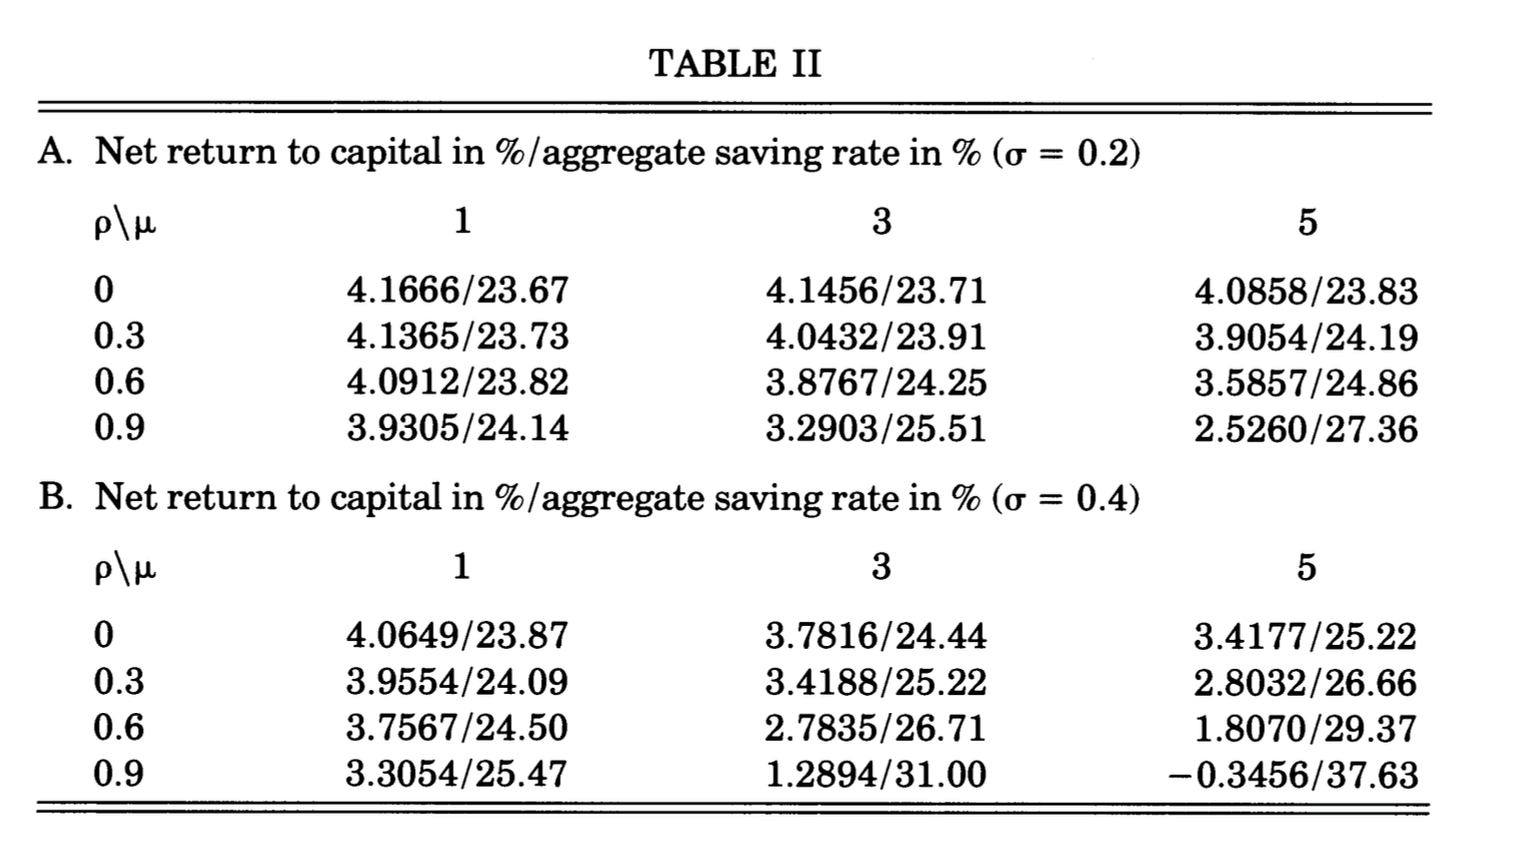
\includegraphics[scale=0.5]{Table-Aiyagari}

\end{document}
